\documentclass{article}
\usepackage{a4wide}
\usepackage{amsmath,graphicx}
\usepackage[colorlinks=true,linkcolor=blue,citecolor=blue]{hyperref}
\usepackage[sort&compress,comma,authoryear]{natbib}
\newcommand{\Prob}[0]{\mbox{Prob}}
\newcommand{\ul}[1]{\underline{#1}}
\newcommand{\ol}[1]{\overline{#1}}
\usepackage{bm}
\usepackage{latexsym}


\title{DEB model description: 'asj'}
%\author{S.A.L.M. Kooijman and K. Lika and S. Augustine and N. Marn and others?}


\begin{document}

\maketitle

This document specifies the typified DEB model 'asj'.
This model belongs to the class of a-models which assumes that type {\cal M} (metabolic) acceleration occurs during part of the life-cycle. 


The 'asj' {\sc deb} model includes a delayed (with respect to birth) type {\cal M} acceleration and is like the 'std' model except that:
\begin{description}
  \item[$\circ$] start of acceleration is delayed with respect to birth till maturity level $E_H^s$ and lasts till metamorphosis at maturity level $E_H^j$
	
  \item[$\circ$] Before and after acceleration: isomorphy
\end{description}
Metamorphosis is still before puberty, so $E_H^b \le E_H^s \le E_H^j \le E_Hp$ and the acceleration factor is $s_{\cal M} = L_j/ L_s$.
This model is a one-parameter extension of the abj-model and reduces to the std-model for $E_H^b = E_H^s = E_H^j$.
This life history is found in \emph{Mnemiopsis} \citep{AuguJasp2014}, \emph{Crassostrea} and \emph{Aplysia}.
Further improvement of data might require a change from abj- to asj-models for quite a few species.


\begin{figure}[htbp]%
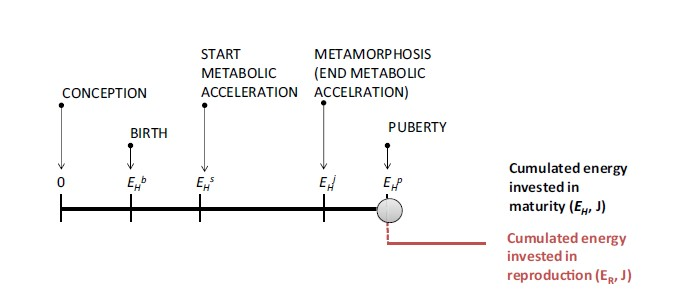
\includegraphics[width=0.9\textwidth]{asj.jpg}%
\caption{\protect\small The life-cycle is structured according to maturity level. Here we have an overview of the asj life-cycle. From \citet{AuguJasp2014}.}%
\label{fig:asj}%
\end{figure}

The following section provides an overiew of how the 'asj' model fits within a wider framework of DEB related models before technically specifying the std model.

\section{Background}


\subsection{Life-stages}

It serves to understand the difference between morphological life-stages and functional lifestage. Morphological life-stage are attributed based on a description of the species or group.
For example an insect might have the following morphological life stages: egg, larva, (sub)imago. 
A bird could have: egg, chick, (immature)adult. 
A human mammal: fetus, baby, child, teenager, adult. 
Something like a cheetah has a fetus, cubs, juveniles and adults. 
There are many reproductive strategies, and some groups have species with a fetus-like development and others who lay eggs. 

So one could make a rather long list of all types of morphological life-stages used to describe different part of the life-cycle across all animal kingdom.
Dynamic energy Budget theory provides a synthetic description of the life-cycle of all animals using a reduced list of functional stages: embryo, juvenile, adult, and imago.
A single model captures the full life-cycle from conception to death and transitions between functional life-stages are construed as switches.

Fetuses and eggs are embryo's: they grow, mature and do not feed. 
Babies, children, cubs, (some) larvae are all "juveniles": the grow, feed and mature but do not yet reproduce.
Sometimes finding out what functional life stage best describes a morphological life-stage is the result of some investigation.

\subsection{A unified energetic basis captures animal biodiversity}

As the number of species grew, for which DEB models were applied to animal taxa (over 3000 from all major phyla as of (2022/02/01) it became evident that the standard DEB model, 'std' required simple extensions for particular taxa, e.g.\ to accommodate larval life stages, foetal development, various forms of metabolic acceleration \cite{Kooy2014}, substantial programmed shrinking (observed for \href{https://fishtreeoflife.org/taxonomy/megacohort/Elopocephalai/}{Elopocephalai} a mega cohort of ray-finned fish that includes eels)  etc.

A typified model can now be selected from a set, see the \textbf{Typified models} page of the DEBwiki: \href{http://www.debtheory.org/wiki/index.php?title=Typified_models}. 
The choice of typified model depends on higher-level classifications, not on the species-level. 
These related models belong to three families \textbf{s} , \textbf{a} and \textbf{h}. 
Their relative frequency within the online AmP database is updated with each new entry: 

The \textbf{s--}models apply to most animal species without larval phases, like birds or some crustaceans. 
Models for mammals are part of this model family but deviate from the standard model by having a fetus, the production of milk mostly by females and a diet-switch of the juvenile at weaning. 
Most mammals also delay start of fetal development during gestation (so-called diapause).

The \textbf{a--}models apply to most species with a larval phase. 
The analysis of data for thousands of animals revealed that these species show metabolic acceleration at, or soon after, birth; 
the end of acceleration frequently coincides with morphological metamorphosis.
\href{https://en.wikipedia.org/wiki/Entognatha}{Enthognaths}, (which include springtails) and arachnids (spiders) are examples of species who can sometimes substantially accelerate their metabolism while they do not have clear larval stages nor morphological metamorphosis.
Since the oldest animal group, the Radiata, and the oldest deuterostomes, the echinoderms, accelerate, it might well be that acceleration became  suppressed in several other groups and this suppression evolved several times in evolution \cite{Kooy2014}. 

%\begin{figure}[htbp]%
%\includegraphics[width=0.9\textwidth]{http://www.bio.vu.nl/thb/deb/deblab/add_my_pet/img/phyla/acceleration_taxa.png}%
%\caption{\protect\small Overview of metabolic acceleration across taxa, from \href{http://www.bio.vu.nl/thb/deb/deblab/add_my_pet/phyla.html}{AmP Phyla overview} (itself an update of \citep{MarqAugu2018}.}%
%\end{figure}
%\label{fig:asj}%


The \textbf{h--}models mostly apply to \href{https://en.wikipedia.org/wiki/Insect}{insects} (also included in the hexapods). Most insects seem to skip the juvenile phase and allocate to reproduction as larvae, which classifies them as adult in DEB terms, while the imago neither grows, nor eats (frequently).
Holometabolic insects insert a pupal phase between the larval and imago phases that behaves like an embryo with a reproduction buffer, where most of the larval structure is first converted to reserve \cite{LlanMarq2015} and imago structure is build from reserve.

Delayed stage transitions are also accounted for in the different model families. 
Most mammals delay start of fetal development during gestation. 
Some bivalves delay the start of metabolic acceleration; 
this phenomenon can prove to be more common with the increase of available data.

\subsection{ressources}

This small movie provides the overview of the related family of DEB models for animals: \url{https://youtu.be/E4ag2-WzhmQ}.


% input to all of the model descriptions
\section{Notation and units}

All if the symbols, and their dimensions, used herein are defined in the \href{https://www.bio.vu.nl/thb/deb/deblab/bib/Kooy2010_n.pdf}{DEB notation document}.
\href{https://www.bio.vu.nl/thb/deb/deblab/add_my_pet/about.html}{The AmP collection} contains  11 related {\sc deb} models.

\section{Specification of the 'std' model}



All models are variations on the standard ('std') model which is specified as follows, where
the environmental variables, temperature $T(t)$ and food density $X(t)$, can change in time $t$.
All models handle environmental variables in the same way:

\vspace{5mm}\noindent{\bf\em Effect of temperature on any rate $\dot{k}$}: {\small
\begin{description}
   \item[Basic: ]  $\frac{\dot{k}(T)} {\dot{k}(T_{\mbox{\tiny ref}})} =  
	    \exp \left( \frac{T_A} {T_{\mbox{\tiny ref}}} - \frac{T_A} {T} \right)$

   \item[Extended: ]  $\frac{\dot{k}(T)} {\dot{k}(T_{\mbox{\tiny ref}})} =  
	    \exp \left( \frac{T_A} {T_{\mbox{\tiny ref}}} - \frac{T_A} {T} \right) 
			\frac{1 + \exp\left(\frac{T_{AL}} {T_{\mbox{\tiny ref}}} - \frac{T_{AL}} {T_L}\right)_+ + 
			          \exp\left(\frac{T_{AH}} {T_H} - \frac{T_{AH}} {T_{\mbox{\tiny ref}}}\right)_+}
	         {1 + \exp \left( \frac{T_{AL}} {T} - \frac{T_{AL}} {T_L} \right)_+ + \exp \left(\frac{T_{AH}} {T_H} - \frac{T_{AH}} {T} \right)_+}$
\end{description}}

\vspace{5mm}\noindent{\bf\em Effect of food on assimilation}: {\small
\begin{description}
  \item if $E_H < E_H^b$, $\dot{p}_X = 0$,  else $\dot{p}_X = f \{\dot{p}_{Xm}\} L^2$ with 
	   $f = \frac{X} {K + X}$ and $K = \frac{\{\dot{J}_{Xm}\}} {\{\dot{F}_m\}}$ and
		 $\{\dot{p}_{Xm}\} = \{\dot{p}_{Am}\}/ \kappa_X$
\end{description}}


\subsection{std model}

The std-model follows from the assumptions as listed in Table \ref{tab:assumptions}.

\begin{table}[tb]\small
\caption[]{\label{tab:assumptions}\protect\small 
  \index{assumptions} The assumptions that specify the standard \hyperref[glos:DEB]{\sc deb}
  model quantitatively. This is a copy of Table 2.4 from \citet{Kooy2010}
	}.

  \rule{16cm}{.1mm}
\begin{itemize}
  
\item[1] The amounts of reserve, structure and maturity are the state variables of the individual; 
  reserve and structure have a constant composition (strong \hyperref[glos:homeostasis]{homeostasis}) and maturity represents information.
  
\item[2] Substrate (food) \hyperref[glos:uptake]{uptake} is initiated (birth) and allocation to maturity is redirected to reproduction (puberty) if maturity reaches certain threshold values.
  
\item[3] Food is converted into reserve and reserve is mobilised at a rate that depends on the \hyperref[glos:state_variable]{state variables} only to fuel all other metabolic processes.
  
\item[4] The embryonic stage has initially a negligibly small amount of structure and maturity (but a substantial amount of reserve).
  The reserve \hyperref[glos:density]{density} at birth equals that of the mother at egg formation (maternal effect).
  Foetuses develop in the same way as embryos in eggs, but at a rate unrestricted by reserve availability.
  
\item[5] The feeding rate is proportional to the surface area of the individual and the food--handling time is independent of food \hyperref[glos:density]{density}.
 
\item[6] The reserve \hyperref[glos:density]{density} \emph{at constant food \hyperref[glos:density]{density}} does not depend on the amount of structure (weak \hyperref[glos:homeostasis]{homeostasis}).
  
\item[7] Somatic \hyperref[glos:maintenance]{maintenance} is proportional to structural volume, but some components (osmosis in aquatic organisms, heating in \hyperref[glos:endotherm]{endotherms}) are proportional to structural surface area.
  
\item[8] Maturity \hyperref[glos:maintenance]{maintenance} is proportional to the level of maturity

\item[9] A fixed fraction of mobilised reserves is allocated to somatic \hyperref[glos:maintenance]{maintenance} plus \hyperref[glos:growth]{growth}, the rest to maturity maintenance plus maturation or reproduction (the $\kappa$-rule).
  
\item[10] The individual does not change in shape during growth (\hyperref[glos:isomorph]{isomorphism}).
  This assumption applies to the standard \hyperref[glos:DEB]{\sc deb} model only.

\end{itemize}
  \rule{16cm}{.1mm}
\end{table}


Within the family of {\sc deb} models, the std-model can be seen as a canonical form.

\vspace{5mm}\noindent{\bf\em Main characteristics}: {\small
\begin{description}
  \item[$\circ$] 1 type of food $X$, 1 type of structure $V$, 1 type of reserve $E$, 1 type of feces $P$ 
	
	\item[$\circ$] 4 minerals (carbon dioxide $C$, water $H$, dioxygen $O$, N-waste $N$); $O$ is not limiting 
	
  \item[$\circ$] 3 life stages (embryo, juvenile, adult) triggered by maturity thresholds
	
	  \subitem $\bullet$ birth is defined as start of assimilation via food uptake 
		
		\subitem $\bullet$ puberty as end of maturation and start of allocation to reproduction
		
	\item[$\circ$] If mobilisation is not fast enough to cover maturity and/or somatic maintenance,
	  rejuvenation and/or some shrinking can occur, but only after use of the reproduction buffer
		
	\item[$\circ$] The reproduction buffer is continuously converted to a spawning buffer, which is instantaneously converted to exported eggs,
	  if the spawning buffer exceeds a density threshold
\end{description}}

\vspace{5mm}\noindent{\bf\em Parameters}: {\small
\begin{description}
  \item[Temperature: ] $T_A$, $T_L$, $T_H$, $T_{AL}$, $T_{AH}$ 
	
	\item[Hazard: ] $\ddot{h}_a$, $s_G$, $\delta_L$, $\dot{h}_J$, $\dot{h}_0$, $\dot{h}_0^e$
	
	\item[Life stage: ] $E_H^b$, $E_H^p$
	
  \item[Core: ] $\{\dot{F}_m\}$, $\{\dot{p}_{Am}\}$, $[\dot{p}_M]$, $\{\dot{p}_T\}$, $\dot{k}_J$, $\dot{k}_J^\prime$, 
	  $\dot{v}$, $[E_G]$, $\kappa$, $\kappa_X$, $\kappa_P$, $\kappa_R$, $[E_R^s]$
		
  \item[Chemical: ] $[M_V]$, 
	  ${\bm d}_{\cal O} = (\begin{array}{cccc} d_X & d_V & d_E & d_P \end{array})$, 
	  ${\bm \mu}_{\cal O} = (\begin{array}{cccc} \ol{\mu}_X & \ol{\mu}_V & \ol{\mu}_E & \ol{\mu}_P\end{array})$,
	  ${\bm n}_{\cal M}$, ${\bm n}_{\cal O}^d$,\\
		  where the chemical coefficients for minerals and (dry) organic compounds are\\
	  ${\bm n}_{\cal M} = \left( 
      \begin{array}{cccc} 
        1 & 0 & 0 & n_{CN}\\ 
			  0 & 2 & 0 & n_{HN}\\ 
        2 & 1 & 2 & n_{ON}\\ 
			  0 & 0 & 0 & n_{NN} 
      \end{array} \right)$ and 
	  $ {\bm n}_{\cal O}^d = \left( 
    \begin{array}{cccc}
      1        & 1        & 1        & 1       \\ 
			n_{HX}^d & n_{HV}^d & n_{HE}^d & n_{HP}^d\\
      n_{OX}^d & n_{OV}^d & n_{OE}^d & n_{OP}^d\\ 
			n_{NX}^d & n_{NV}^d & n_{NE}^d & n_{NP}^d 
    \end{array} \right)$.\\ 
		If the N-waste is ammonia, we have $n_{CN} = 0$, $n_{HN} = 3$, $n_{ON} = 0$, $n_{NN} = 1$.
\end{description}}


\vspace{5mm}\noindent{\bf\em Help quantities (for the specification of changes in state)}: {\small
\begin{description}
  \item [wet/dry mass: ]
	  The chemical coefficients of wet organic mass $n_{*_1 *_2}^w$ relate to that of dry mass $n_{*_1 *_2}^d$ 
		  for $*_1 \in \{H, O\}$ and $*_2 \in \{X, V, E, P\}$ as 
			$n_{H *_2}^w = 2 x_{*_2} + n_{H *_2}^d$ and $n_{O *_2}^w = x_{*_2} + n_{O *_2}^d$, 
			while $n_{C *_2}^w = n_{C *_2}^d$ and $n_{N *_2}^w = n_{N *_2}^d$, 
			where $x_{*_2} = \frac{1 - d_{*_2}^d/ d_{*_2}^w} {18}$, 
		  while $d_{*_2}^w \simeq 1$\,g/cm$^3$.\\
		%The molecular weights of dry mass are $w_{*_2}^d = 12 n_{C *_2}^d + n_{H *_2}^d + 16 n_{O *_2}^d + 14 n_{N *_2}^d$.\\
    %The molecular weights of wet mass relate to that of dry mass as $w_{*_2}^w =  w_{*_2}^d + 18 x_{*_2}$.\\

  \item[mass fluxes: ] $\dot{\bm J}_{\cal O} = (
		\begin{array}{cccc} 
	     \dot{J}_X & \dot{J}_V & (\dot{J}_E + \dot{J}_{E_R}) &  \dot{J}_P 
	  \end{array})$
    relate to energy fluxes 
		$\dot{\bm p} = \left(\begin{array}{ccc} \dot{p}_A & \dot{p}_D & \dot{p}_G \end{array} \right)$, as
    $\dot{\bm J}_{\cal O} = {\bm \eta}_{\cal O} \dot{\bm p}$ with 
    ${\bm \eta}_{\cal O} = 
		  \left( \begin{array}{ccc} 
        -\frac{1} {\kappa_X \ol{\mu}_X}       & 0                       & 0\\ 
			  0                                     & 0                       & \frac{\kappa_G} {\ol{\mu}_V}\\ 
        \frac{1} {\ol{\mu}_E}                 & - \frac{1} {\ol{\mu}_E} & - \frac{1} {\ol{\mu}_E}\\ 
        \frac{\kappa_P} {\kappa_X \ol{\mu}_P} & 0                       & 0 
      \end{array} \right)$
	  and $\kappa_G = \ol{\mu}_V \frac{[M_V]} {[E_G]}$
	
  \item[assimilation: ] $\dot{p}_A = \kappa_X \dot{p}_X$ 

	\item[somatic maintenance: ] $\dot{p}_S = [\dot{p}_S] L^3$.		
	  If $E_H < E_H^b$, $[\dot{p}_S] = [\dot{p}_M]$, else $[\dot{p}_S] = [\dot{p}_M]  + \{\dot{p}_T\}/ L$
			
	\item[maturity maintenance: ] if $(1 - \kappa) \dot{p}_C > \dot{k}_J E_H$ (no rejuvenation), 
	  $\dot{p}_J = \dot{k}_J E_H$, else $\dot{p}_J = \dot{k}_J^\prime E_H$
		
	\item[mobilization: ] $\dot{p}_C = E (\dot{v}/ L - \dot{r})$. 
	  If $[E] \ge \frac{[\dot{p}_S] L} {\dot{v} \kappa}$ (no shrinking), 
		  $\dot{r} = \frac{[E] \dot{v}/ L - [\dot{p}_S]/ \kappa} {[E] + [E_G]/ \kappa}$, 
		else if $E_R > 0$, $\dot{r} = 0$, or if $E_R \le 0$, 
		  $\dot{r} = \frac{[E] \dot{v}/ L - [\dot{p}_S]/ \kappa} {[E] + [E_G] \kappa_G/ \kappa}$ (shrinking)

	\item[growth: ] $\dot{p}_G = \kappa \dot{p}_C - \dot{p}_S$, 
	  but if $\kappa \dot{p}_C < \dot{p}_S$ and $E_R > 0$: $\dot{p}_G = 0$

  \item[maturation/reproduction: ] $\dot{p}_R = (1 - \kappa) \dot{p}_C - \dot{p}_J$, 
	  but if $(1 - \kappa) \dot{p}_C < \dot{p}_J$ and $E_R > 0$: $\dot{p}_R = 0$

	\item[dissipation: ] if $E_H < E_H^p$, $\dot{p}_D = \dot{p}_S + \dot{p}_J + \dot{p}_R$,  
	  else $\dot{p}_D = \dot{p}_S + \dot{p}_J + (1 - \kappa_R) \dot{p}_R$
\end{description}}
		
		
\vspace*{5mm}\noindent{\bf\em Initial states}: {\small
$L(0) = 0$, $E_H(0) = 0$, $E_R(0) = 0$, $\ddot{q}(0) = 0$, $\dot{h}_A(0) = 0$ and $E(0) = E_0$ 
  such that $[E](a_b)$ equals that of mother at egg production}

\vspace*{5mm}\noindent{\bf\em Changes in state}: {\small
\begin{description}
  \item[structure: ] $\frac{d} {dt} L = L \dot{r}/ 3$.
		So, initial change is $\frac{d} {dt} L(0) = \dot{v}/ 3$
			
  \item[reserve:] If $E_H < E_H^b$ (embryo), $\frac{d} {dt} [E] = - [E] \dot{v}/ L$, else $\frac{d} {dt} [E] = (\{\dot{p}_{Am}\} f - [E] \dot{v})/ L$
	
  \item[maturity:] If $E_H < E_H^p$ (embryo or juvenile), $\frac{d} {dt} E_H = \dot{p}_R$, else $\frac{d} {dt} E_H = 0$. 
	  However, if $\dot{p}_J < 0$ and $E_R = 0$ (rejuvenation), 
	    $\frac{d} {dt} E_H = \dot{p}_J^\prime$ with $\dot{p}_J^\prime = \min(0, \dot{p}_J \dot{k}_J^\prime/ \dot{k}_J)$
			
  \item[buffer:] If $E_H = E_H^p$ (adult), $\frac{d} {dt} E_R = \dot{p}_R - \dot{p}_J^\prime - \dot{p}_G^\prime$, 
	  else ($E_H < E_H^p$) $\frac{d} {dt} E_R = 0$.
		If adult and $E_R > 0$, $\dot{p}_G^\prime = \max(0, [\dot{p}_S] L^3 - \kappa \dot{p}_C)$, 
		  else ($E_R \le 0$) $\dot{p}_J^\prime = 0$ and $\dot{p}_G^\prime = 0$.
		The buffer is partitioned as $E_R = E_R^0 + E_R^1$, where $E_R^0$ converts, for positive $E_R^0$, to $E_R^1$ at rate
			$\dot{p}_R^{\max} = \frac{1 - \kappa} {\kappa} L^3 \frac{[E_G] \dot{v}/L + [\dot{p}_S]} {1 + g} - \dot{p}_J$ and 
			$g = \frac{[E_G] \dot{v}}{\kappa \{\dot{p}_{Am}\}}$.
			
  \item[hazard:] $\dot{h} = \dot{h}_A + \dot{h}_X + \dot{h}_B + \dot{h}_P$
	
	  \subitem $\bullet$ aging: 
			$\frac{d} {dt} \ddot{q} = (\ddot{q} \frac{L^3} {L_m^3} s_G + \ddot{h}_a) e (\frac{\dot{v}} {L} - \dot{r}) - \dot{r} \ddot{q}; \quad 
      \frac{d} {dt} \dot{h}_A = \ddot{q} - \dot{r} \dot{h}_A$
				
	  \subitem $\bullet$ starving (food): If $E_H < E_H^b$, $\dot{h}_X = 0$, else if $\dot{p}_C   < \frac{\dot{k}_J E_H} {1 - \kappa}$, 
			$\dot{h}_X = \dot{h}_J (1 - \frac{\dot{p}_C (1 - \kappa)} {\dot{k}_J E_H})$.\\
			\hspace*{9mm} Let $L_0$ be the length at which $\dot{r} = 0$ for the last time.\\ 
			\hspace*{9mm} If $L = \delta_L L_0$, $h_X \, dt = \infty$ (instant death due to shrinking)
				
		\subitem $\bullet$ accidental (background): If $E_H < E_H^b$, $\dot{h}_B = \dot{h}_B^{0b}$, else $\dot{h}_B = \dot{h}_B^{bi}$; both constant
			
	  \subitem $\bullet$ thinning (predation): If $E_H \ge E_H^b$, $\dot{h}_P = \frac{2} {3} \dot{r}$, else $\dot{h}_P = 0$	
\end{description}}
	
\vspace{5mm}\noindent{\bf\em Input/output fluxes}: {\small
\begin{description}
  \item[food: ] $\dot{J}_X = \frac{\dot{p}_A} {\kappa_X \ol{\mu}_X}$ 
		
  \item[feces: ] $\dot{J}_P = \frac{\kappa_P \dot{p}_A} {\kappa_X \ol{\mu}_P}$
		
  \item[eggs: ] If $E_R^1 = [E_R^s] L^3$: $\dot{R}\,dt = \kappa_R [E_R^s] L^3/ E_0$ eggs are produced and $E_R^1$ is set to $0$ 
		
  \item[minerals: ] $\dot{\bm J}_{\cal M} = - {\bm n}_{\cal M}^{-1} {\bm n}_{\cal O}^w \dot{\bm J}_{\cal O}$, where 
		$\dot{\bm J}_{\cal M} = (\begin{array}{cccc} \dot{J}_C  & \dot{J}_H & \dot{J}_O  & \dot{J}_N \end{array})$
			
	\item[heat: ] $\dot{p}_{T+} = - \ol{\bm \mu}_{\cal O}^T \dot{\bm J}_{\cal O}$
		
	\item[death: ] at death, $[M_V] L^3$ moles of structure and $(E + E_R)/ \ol{\mu}_E$ moles of reserve become available in the environment
\end{description}}



\bibliographystyle{apalike}
\bibliography{debmodels}

\end{document}